% (The MIT License)
%
% Copyright (c) 2023-2024 Yegor Bugayenko
%
% Permission is hereby granted, free of charge, to any person obtaining a copy
% of this software and associated documentation files (the 'Software'), to deal
% in the Software without restriction, including without limitation the rights
% to use, copy, modify, merge, publish, distribute, sublicense, and/or sell
% copies of the Software, and to permit persons to whom the Software is
% furnished to do so, subject to the following conditions:
%
% The above copyright notice and this permission notice shall be included in all
% copies or substantial portions of the Software.
%
% THE SOFTWARE IS PROVIDED 'AS IS', WITHOUT WARRANTY OF ANY KIND, EXPRESS OR
% IMPLIED, INCLUDING BUT NOT LIMITED TO THE WARRANTIES OF MERCHANTABILITY,
% FITNESS FOR A PARTICULAR PURPOSE AND NONINFRINGEMENT. IN NO EVENT SHALL THE
% AUTHORS OR COPYRIGHT HOLDERS BE LIABLE FOR ANY CLAIM, DAMAGES OR OTHER
% LIABILITY, WHETHER IN AN ACTION OF CONTRACT, TORT OR OTHERWISE, ARISING FROM,
% OUT OF OR IN CONNECTION WITH THE SOFTWARE OR THE USE OR OTHER DEALINGS IN THE
% SOFTWARE.

\documentclass{article}
\usepackage{../lecture-notes/notes}
\usepackage{amsmath}
\usepackage{relsize}
\newcommand*\thetitle{Clone Coverage}
\begin{document}

% read this, it's one of the most recent:
% https://www.computer.org/csdl/proceedings-article/icse/2024/021700b006/1V5BlfnaOpG

\plush{\lnTitlePage{11}{24}{ynPTEzDTutc}}

\lnQuote
  [Edward Yourdon]
  {edward-yourdon}
  {Whenever possible, we wish to maximize \ul{fan-in} during the design process. Fan-in is the \textit{raison d'\^{e}tre} of modularity: Each instance of multiple fan-in means that some \ul{duplicate code} has been avoided.}
  {yourdon1979structured}

\lnQuote
  [Robert C. Martin]
  {robert-martin}
  {Duplication is the \ul{primary enemy} of a well-designed system.}
  {martin2008clean}

\lnQuote
  [Qurat Ul Ain]
  {qurat-ul-ain}
  {If a bug is identified in one segment of code, all the similar segments need to be \ul{checked} for the same bug. Consequently, code duplication may lead to bug propagation that significantly affects the maintenance cost.}
  {ain2019}

\lnQuote
  [Rainer Koschke]
  {rainer-koschke}
  {The problem with code cloning is that errors in the original must be fixed in every copy. Other kinds of maintenance changes, for instance, extensions or adaptations, must be applied \ul{multiple times}, too. Yet, it is usually not documented \ul{where} code was copied.}
  {bellon2007}

\pptBanner{Motivating Example (part I)}
\begin{multicols}{2}
Before (\textcolor{red}{wrong}):\par
{\small\begin{ffcode}
printf("Hi, %s!", getName(42));
printf("Hi, %s!", getName(7));
printf("Hi, %s!", getName(55));
\end{ffcode}
}
\par\columnbreak\par
After (\textcolor{orange}{better}):\par
{\small\begin{ffcode}
sayHello(42);
sayHello(7);
sayHello(55);

void sayHello(int id) {
  var n = getName(id);
  printf("Hi, %s!", n);
}
\end{ffcode}
}
\end{multicols}
\plush{}

\pptBanner{Motivating Example (part II)}
\begin{multicols}{2}
Before (\textcolor{orange}{still not ideal}):\par
{\small\begin{ffcode}
sayHello(42);
sayHello(7);
sayHello(55);

void sayHello(int id) {
  var n = getName(id);
  printf("Hi, %s!", n);
}
\end{ffcode}
}
\par\columnbreak\par
After (\textcolor{green}{perfect}):\par
{\small\begin{ffcode}
var users = [42, 7, 55];
for (id : users) {
  sayHello(id);
}

void sayHello(int id) {
  var n = getName(id);
  printf("Hi, %s!", n);
}
\end{ffcode}
}
\end{multicols}
\plush{}

\lnQuote
  [Brenda S. Baker]
  {brenda-baker}
  {Two lines of code are considered to be identical if they contain the same \ul{sequence of characters} after removing comments and white space; the \ul{semantics} of the program statements are not analyzed.}
  {baker1993}

\plush{
  \pptBanner{Up to 38\% of lines are involved in duplicates}
  \begin{multicols}{2}
  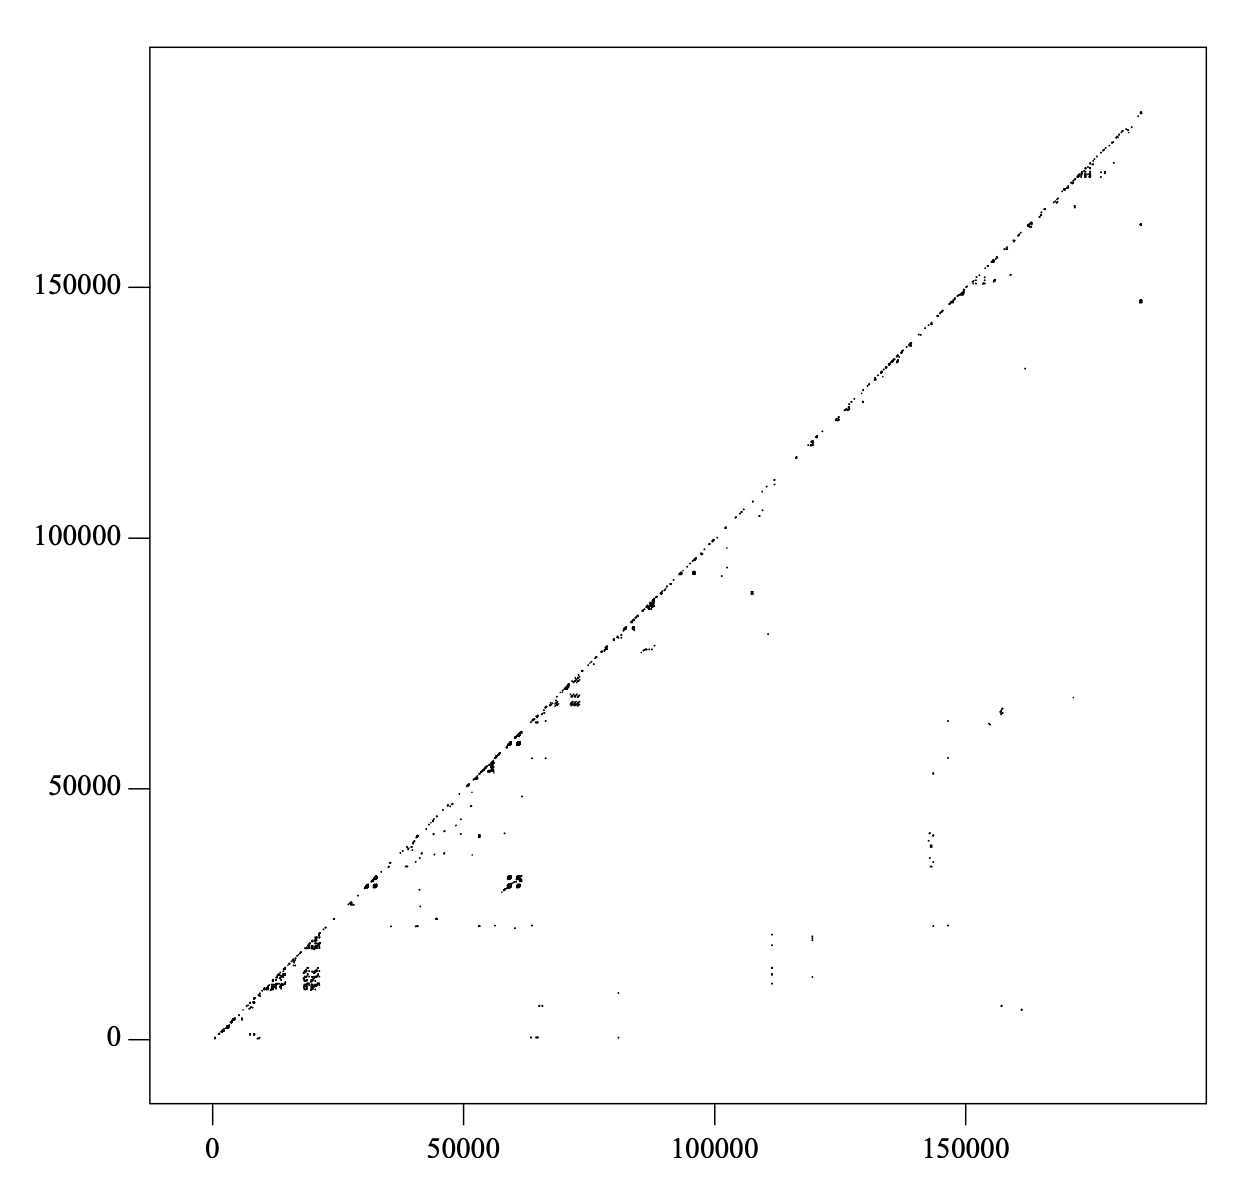
\includegraphics[width=.9\columnwidth]{scatter.png}
  \par\columnbreak\par
  ``The plots are dense near the main diagonal, implying
  that most copies tend to occur \ul{fairly locally}, e.g. within the
  same file or module. However, certain line segments occur
  away from the main diagonal; it would be interesting to
  investigate why the corresponding sections of code are
  duplicated.''
  \lnSource{baker1993}
  \end{multicols}}

\lnQuote
  [Andy Hunt]
  {andy-hunt}
  {\textbf{Don't Repeat Yourself (DRY)}: Every piece of knowledge must have a \ul{single}, unambiguous, authoritative representation within a system.}
  {hunt1999pragmatic}

\lnQuote
  [Kent Beck]
  {kent-beck}
  {\textbf{The Rule of Three}: The \ul{first} time you do something, you just do it. The \ul{second} time you do something similar, you wince at the duplication, but you do the duplicate thing anyway. The \ul{third} time you do something similar, you refactor.}
  {fowler1999refactoring}

\lnQuote
  [Yoshiki Higo]
  {yoshiki-higo}
  {Code-clone analysis is a good vehicle to \ul{quantitatively} understand the differences and improvements between two versions of the same software system}
  {livieri2007}

\lnQuote
  [Wasi Haider Butt]
  {wasi-haider-butt}
  {We identified and analyzed 26 Code Clone Detection (CCD) tools, i.e., 13 existing and 13 proposed/developed. Moreover, 62 open-source subject systems whose source code is utilized for the CCD are presented.}
  {ain2019}

\pptBanner{Type-1: Exact Clone}
\begin{multicols}{2}
Original:\par
{\small\begin{ffcode}
printf("Hi, %s\n", name(42));
\end{ffcode}
}
Clone:\par
{\small\begin{ffcode}
// Here we print a message
// to the console for a user
printf(
  "Hi, %s\n",
  name(42)
);
\end{ffcode}
}
\par\columnbreak\par
Identical code segments except for changes in comments, layouts and whitespaces.
\end{multicols}
\plush{}

\pptBanner{Type-2: Parameterized Clone}
\begin{multicols}{2}
Original:\par
{\small\begin{ffcode}
var n = name(42);
printf("Hi, %s\n", n);
\end{ffcode}
}
Clone:\par
{\small\begin{ffcode}
String name = name(42);
printf("Hi, %s\n", name);
\end{ffcode}
}
\par\columnbreak\par
Code segments which are syntactically or structurally similar other than changes in comments, identifiers, types, literals, and layouts.
\end{multicols}
\plush{}

\pptBanner{Type-3: Gapped Clone}
\begin{multicols}{2}
Original:\par
{\small\begin{ffcode}
printf("Hi, %s\n", name(42));
\end{ffcode}
}
Clone:\par
{\small\begin{ffcode}
var msg = "Hi, %s\n";
var n = name(42);
printf(msg, n);
\end{ffcode}
}
\par\columnbreak\par
Copied pieces with further modification such as addition or removal of statements and changes in whitespaces, identifiers, layouts, comments, and types but outcomes are similar.
\end{multicols}
\plush{}

\pptBanner{Type-4: Semantic Clone}
\begin{multicols}{2}
Original:\par
{\small\begin{ffcode}
printf("Hi, %s\n", name(42));
\end{ffcode}
}
Clone:\par
{\small\begin{ffcode}
var s = sprintf(
  "Hi, %s\n",
  name(42));
print(s);
\end{ffcode}
}
\par\columnbreak\par
More than one code segments that are functionally similar but implemented by different syntactic variants.
\end{multicols}
\plush{}

\plush{
  \pptBanner{Clones in Linux Kernel}
  \pptPic{.9}{clones.png}\par
  \lnSource{casazza2001identifying}}

\plush{
  \pptBanner{Methods of clone detection:}
  \begin{enumerate}
    \item Using text
    \item Using tokens
    \item Using metrics
    \item Using ``tree matching''
    \item Using Program Dependency Graphs (PDG)
    \item Using Machine Learning (ML)
    \item Large Language Models (LLM)
  \end{enumerate}}

\lnQuote
  [Jens Krinke]
  {jens-krinke}
  {For the three Java systems studied, the following results were found: 1)~cloned code is usually \ul{older} than non-cloned code, 2)~cloned code in a file is usually older than the non-cloned code in the same file. Both results suggest that cloned code is \ul{more stable} than non-cloned code.}
  {krinke2011}

\plush{
  \pptBanner{These tools can help detecting duplicate code:}
  \begin{enumerate}
    \item IntelliJ IDEA by JetBrains
    \item Copy/Paste Detector (\href{https://pmd.sourceforge.io/pmd-5.5.2/usage/cpd-usage.html}{CPD}) by PMD for Java
    \item SonarQube
    \item \href{http://www.semdesigns.com/products/clone/}{CloneDR} by Semantic Designs
    \item \href{https://simian.quandarypeak.com/download/}{Simian} by Quandary Peak Research
  \end{enumerate}}

\plush{\pptBanner{Simian 4.0.0}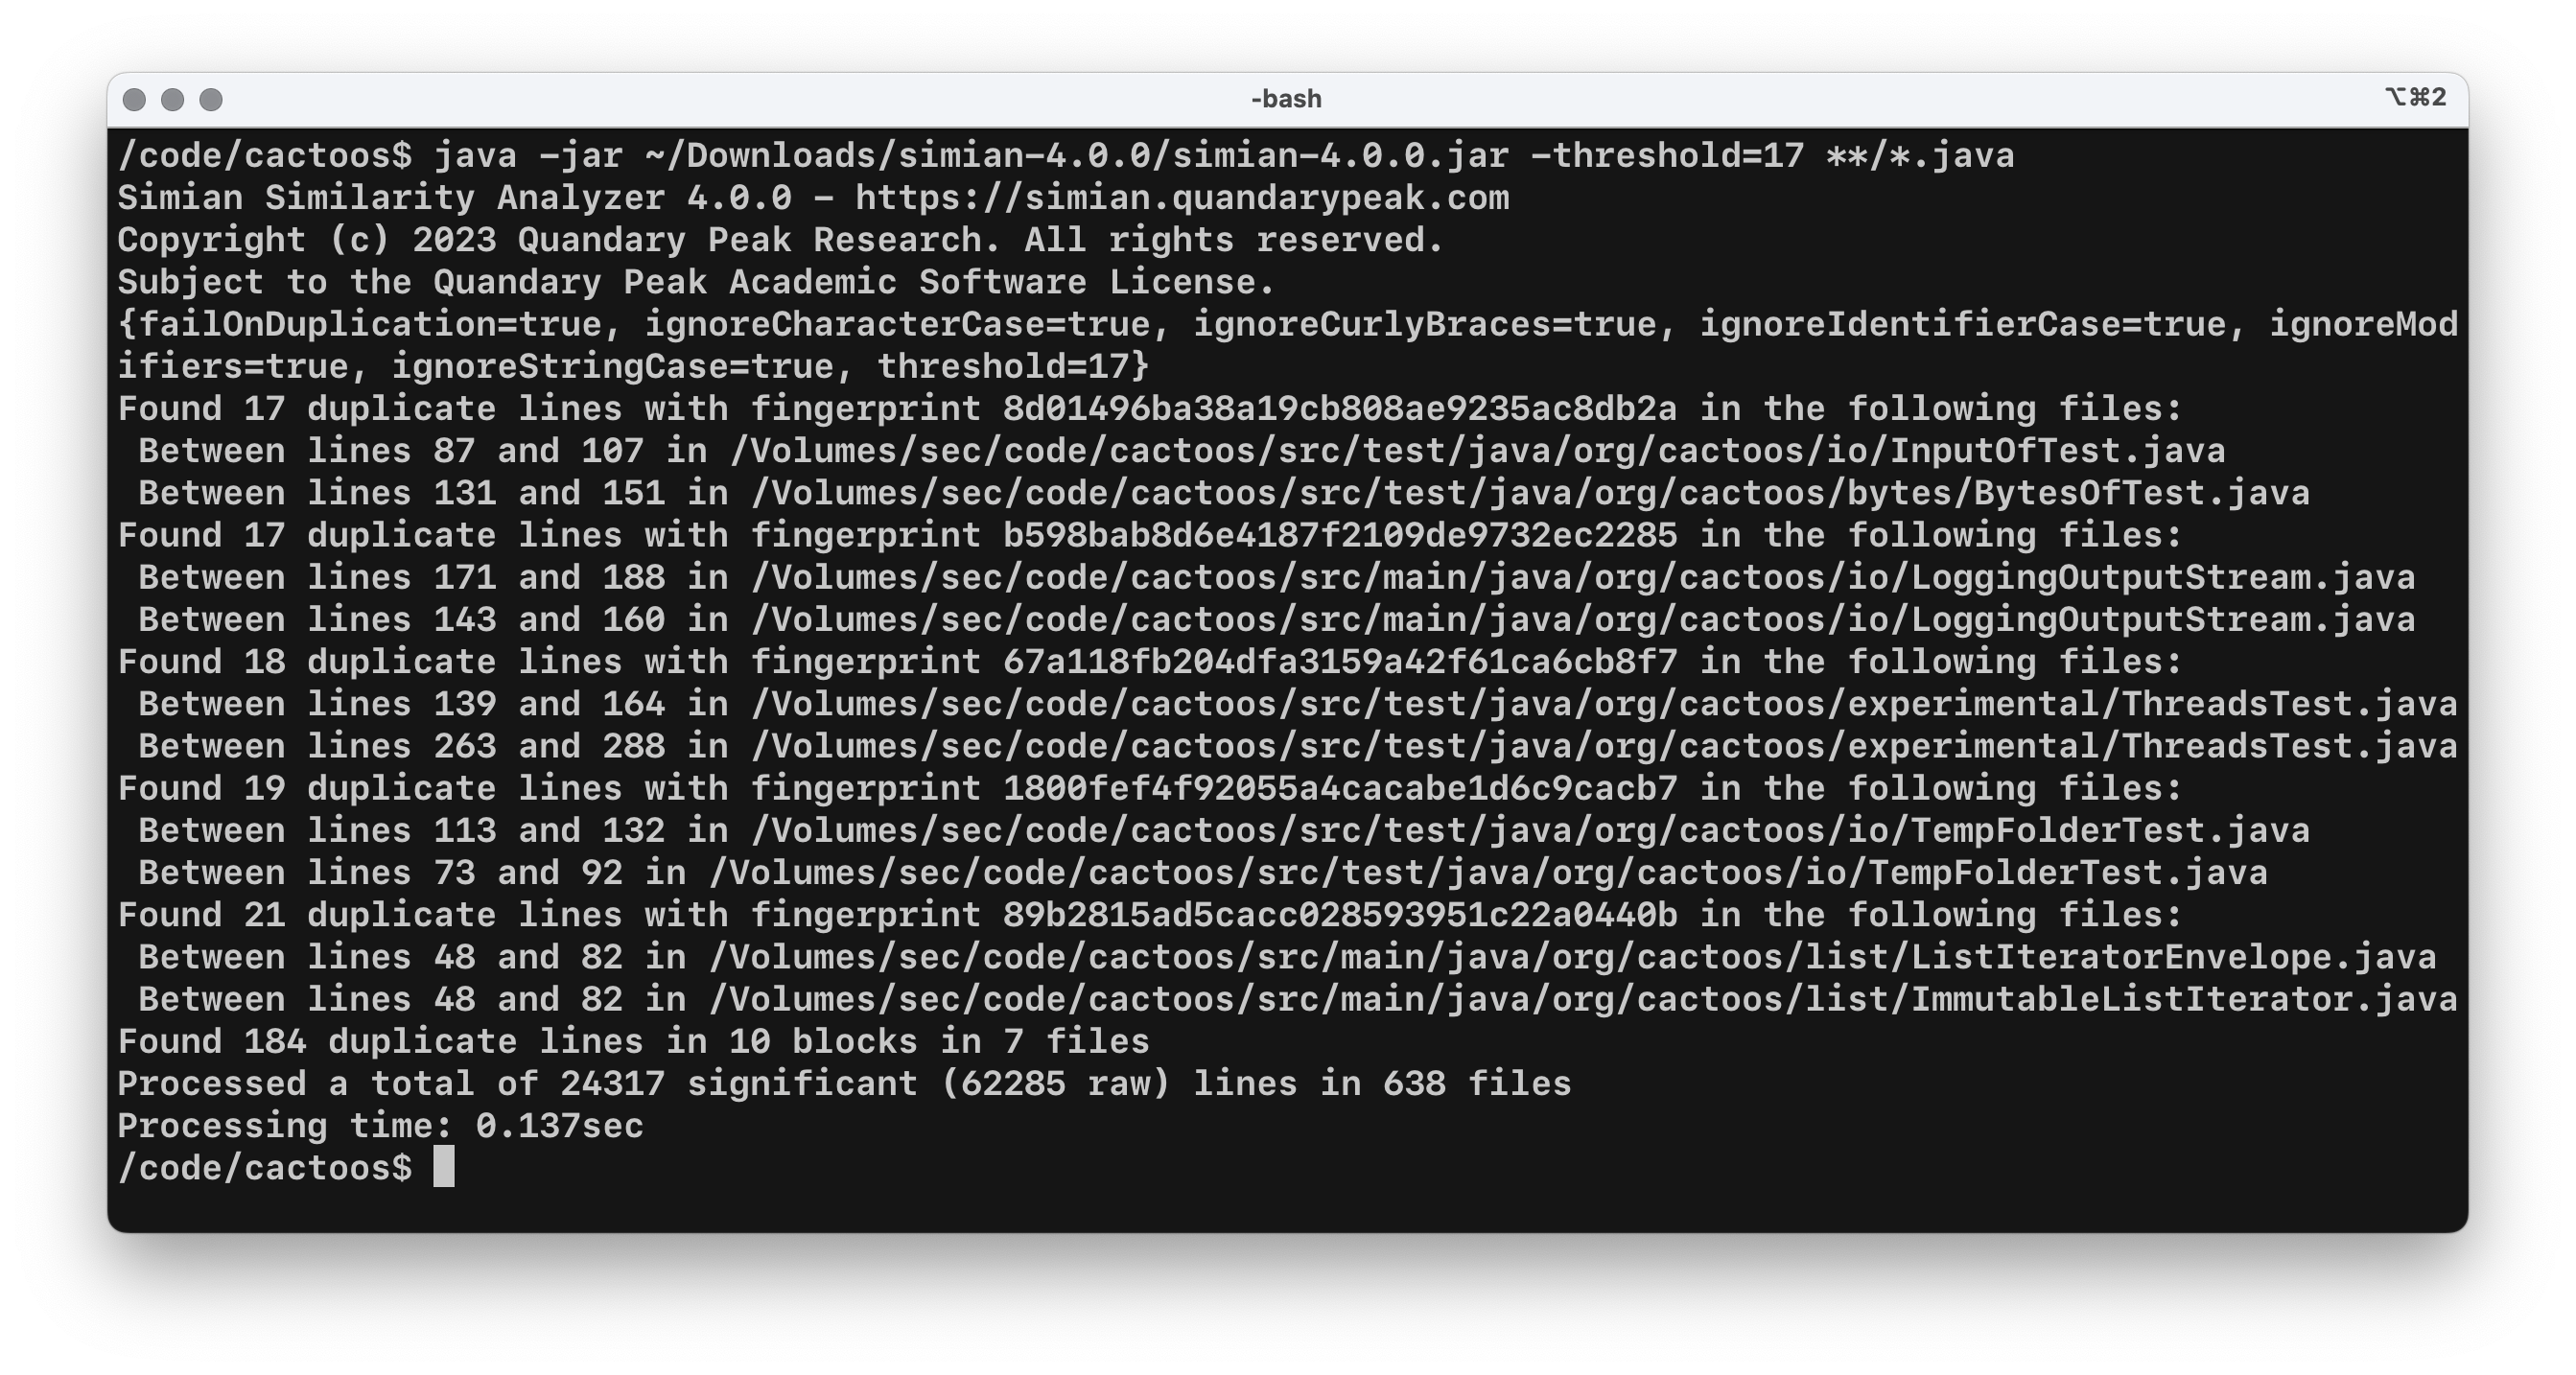
\includegraphics[width=.9\textwidth]{simian.png}}

\plush{
  \pptBanner{How Effective LLMs Are?}
  \begin{multicols}{2}
  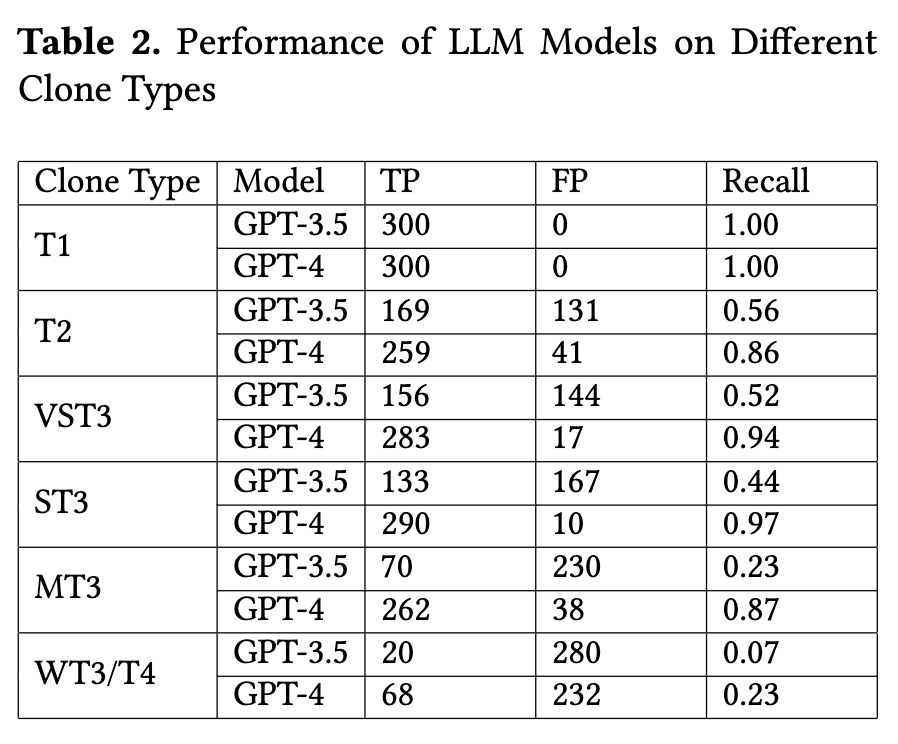
\includegraphics[width=.9\columnwidth]{gpt-recall.png}
  \par\columnbreak\par
  ``A correlation was observed between the GPTs' accuracy at identifying code clones and code similarity, with both GPT models exhibiting \ul{low effectiveness} in detecting the most complex Type-4 code clones.''
  \lnSource{zhang2024assessing}
  \end{multicols}}

\end{document}
